\documentclass [12pt,twoside]{article}
\usepackage{setspace}
\setstretch{1.1}
\usepackage[utf8]{inputenc}
\usepackage[T1]{fontenc}
\usepackage{tabularx}
\usepackage{array}

%Page margins, header and footer positions
\usepackage{geometry}
 \geometry{
 a4paper,
 total={210mm,297mm},
 left=25mm,
 right=25mm,
 top=30mm,
 bottom=25mm,
 headsep=7mm}

\interfootnotelinepenalty=10000

%To display filling dots in the TOC for all entries
\usepackage[titles]{tocloft}
\renewcommand{\cftsecleader}{\cftdotfill{\cftdotsep}}

%Define new header and footer style
\usepackage{fancyhdr}

\pagestyle{fancy}
\fancyhf{}
\lhead{\color{Gray}{\small{CodeKataBattle project - Annechini, Filippi, Fiorentini}}}
\rfoot{\textcolor{Gray}{\thepage}}
\renewcommand{\headrulewidth}{0pt}

%PACKAGES
\usepackage{wasysym}
\usepackage{pifont}

\newcommand{\supported}{\ding{52}\xspace}
\newcommand{\unsupported}{\ding{55}\xspace}
\newcommand{\partsupported}{\textcolor{black!40}{\ding{52}}\xspace}
\newcommand{\lowsupported}{\textcolor{black!20}{\ding{52}}\xspace}
\newcommand{\unknowsupported}{\textbf{?}\xspace}


%Change monospaced font
\renewcommand{\ttdefault}{lmtt}

%tables
\usepackage{tabu}
\usepackage{tabularx}
\usepackage{ltablex}
\usepackage{longtable}
\usepackage{float} % To allow the use of H modifier in long tables

%landscape mode
\usepackage{pdflscape}
\usepackage{rotating}
\usepackage{caption}

%make landscape mode be sensitive to even and odd pages
%start
\def\myrotate{\ifodd\c@page\else-\fi 90}
\makeatletter
\global\let\orig@begin@landscape=\landscape%
\global\let\orig@end@landscape=\endlandscape%
\gdef\@true{1}
\gdef\@false{0}
\gdef\landscape{%
    \global\let\within@landscape=\@true%
    \orig@begin@landscape%
}%
\gdef\endlandscape{%
    \orig@end@landscape%
    \global\let\within@landscape=\@false%
}%
\@ifpackageloaded{pdflscape}{%
    \gdef\pdf@landscape@rotate{\PLS@Rotate}%
}{
    \gdef\pdf@landscape@rotate#1{}%
}
\let\latex@outputpage\@outputpage
\def\@outputpage{
    \ifx\within@landscape\@true%
        \if@twoside%
            \ifodd\c@page%
                \gdef\LS@rot{\setbox\@outputbox\vbox{%
                    \pdf@landscape@rotate{-90}%
                    \hbox{\rotatebox{90}{\hbox{\rotatebox{180}{\box\@outputbox}}}}}%
                }%
            \else%
                \gdef\LS@rot{\setbox\@outputbox\vbox{%
                    \pdf@landscape@rotate{+90}%
                    \hbox{\rotatebox{90}{\hbox{\rotatebox{0}{\box\@outputbox}}}}}%
                }%
            \fi%
        \else%
            \gdef\LS@rot{\setbox\@outputbox\vbox{%
                \pdf@landscape@rotate{+90}%
                \hbox{\rotatebox{90}{\hbox{\rotatebox{0}{\box\@outputbox}}}}}%
            }%
        \fi%
    \fi%
    \latex@outputpage%
}
\makeatother
%end

%graphics
\usepackage{graphicx}
\usepackage[dvipsnames, table]{xcolor}

%code
\usepackage{minted}
\usemintedstyle{borland}

%Other
\usepackage{ifthen}
\usepackage{xspace}
\usepackage{enumitem}
\usepackage{amssymb}
\usepackage[pdftex,colorlinks=false]{hyperref}
\newcommand{\comment}[1]{{\color{Red}$\blacktriangleright$ Comment: #1 $\blacktriangleleft$}}


% Some utilities\ldots
% Common abbrev. are set as commands to ensure proper spacing after the dot
\RequirePackage{xspace}
\newcommand{\ie}{i.e.\@\xspace}
\newcommand{\aka}{a.k.a.\@\xspace}
\newcommand{\Cf}{Cf.\@\xspace}
\newcommand{\eg}{e.g.\@\xspace}
\newcommand{\etc}{etc.\@\xspace}
\newcommand{\wrt}{w.r.t.\@\xspace}

\date{}

\begin{document}
%TITLE PAGE

\begin{titlepage}

%LOGO
{\begin{table}[t!]
\centering
\begin{tabu} to \textwidth { X[3,c,m]}
    
\includegraphics[scale=0.5]{Images/PolimiLogo} 
\end{tabu}
~\\ [2cm]
\begin{tabu} to \textwidth {X[2,l,m] }
    \textcolor{Black}{\textbf{\small{CodeKataBattle - Annechini Alessandro, Filippi Nicole, Fiorentini Riccardo}}}
\end{tabu}
\end{table}}~\\ [5cm]

%TITLE 

\begin{flushleft}
\centering
%Replace the text string with your title
{\textcolor{Black}{\textbf{\Huge{Requirement Analysis and\\ Specification
        Document}}}} \\ [1cm]
\end{flushleft}

~\\[2cm]

%Define deliverable specific info
%Replace cell contents where needed
\begin{table}[h!]
\begin{tabu} to \textwidth { X[0.22,r,p] X[0.75,l,p] }
\hline
\textbf{Deliverable:} & RASD\\
\textbf{Title:} & Requirement Analysis and Specification Document \\
\textbf{Authors:} & Annechini Alessandro, Filippi Nicole, Fiorentini Riccardo\\
\textbf{Version:} & 1.0 \\ 
\textbf{Date:} & 20-December-2023 \\
\textbf{Download page:} & https://github.com/RiccardoFiorentini/AnnechiniFilippiFiorentini\\
\hline
\end{tabu}
\end{table}

\end{titlepage}



\setcounter{page}{2}


%------------------------------------------------------------------------------------------------------------------------------------------------
\newpage
%\addcontentsline{toc}{section}{Table of Contents}
\tableofcontents
\newpage

%------------------------------------------------------------------------------------------------------------------------------------------------
\clearpage
{\color{Black}{\section{Introduction}}}
\label{sect:introduction}
\subsection{Purpose}
The objective of this Requirements Analysis and Specification Document (RASD) is to delineate the foundational framework for the proposed CodeKataBattle platform (CKB). This comprehensive document will thoroughly detail the functional and non-functional requisites of CKB while outlining system's constraints and boundaries. Primarily, this RASD serves as a directive for the development team tasked with implementing the specified requirements. Simultaneously, it acts as a contractual foundation for stakeholders and end-users, ensuring clarity and alignment between expectations and system capabilities. As such, precision in terminology is important, with explicit definitions provided to enhance mutual understanding. \\
The CKB platform introduces a revolutionary approach to enhancing students' software development proficiency through collaborative training in code kata exercises. Oriented towards creating a competitive yet supportive learning environment. Educators are enabled to construct engaging challenges for students from the platform. These challenges involve teams of students competing to demonstrate and refine their coding skills.

\subsubsection{Goals}
Here are the goals to achieve by implementing the CodeKataBattle (CKB) software:
\begin{table}[h]
    \centering
    \begin{tabular}{|l|l|}
        \hline
        G1 & Educator can create tournaments and battles setting all the necessary parameters and\\& badges \\
        \hline
        G2 & Student can complete battles on their own or in groups by providing their code \\
        \hline
        G3 & Educator that creates a tournament can allow other educators to add battles to the\\&tournament\\
        \hline
        G4 & Students and educators can see the list of ongoing and terminated tournaments and\\&the corresponding rank \\
        \hline
        G5 & Students and educators can see the current rank of every battle they are involved in \\
        \hline
        G6 & Educator can go through the sources produced by a team and manually assign a score \\
        \hline
        G7 & Educators and students can visualize all badges and every student’s collected badges \\
        \hline
    \end{tabular}
    \caption{Goals of the system}
    \label{tab:goals}
\end{table}

\subsection{Scope}
In the fast-evolving landscape of today's technological era, the demand for adept software developers continues to rise. As the significance of collaborative learning and practical skill development becomes increasingly apparent, educational platforms are crucial in shaping the next generation of software engineers. \\
CodeKataBattle (CKB) emerges as an innovative solution, providing a dynamic platform to practice their software development skills collaboratively. In a society where real-world coding challenges and industry-relevant practices are fundamental, CKB bridges the gap between theoretical knowledge and practical application. CKB not only proves instrumental in individual skill enhancement but also promotes a sense of healthy competition. This platform aligns with the contemporary need for hands-on, team-oriented learning experiences.
\\ CKB serves as a vital tool in preparing students for the challenges of today's technology-driven society, where adaptability and collaborative problem-solving are key components of success.
\subsubsection{Description of the system}
CKB is a project aimed to help people to learn how to code but also to improve their software development skills, offering a dynamic and interactive environment for users to engage in collaborative learning. It supports two types of users:
\begin{itemize}
  \item Students
  \item Educators
\end{itemize}
The platform facilitates the creation and management of code kata battles, where students can compete against each other to solve programming exercises in lots of different languages of choice, 
either by themselves or joining a team.  \\
Educators, creating code kata battles, challenge teams of students to compete against each other with diverse coding scenarios, allowing students of proving and improving not just their coding abilities but also their collaboration abilities by working in teams. \\
Each battle follows a structured timeline from registration to final submission, with GitHub integration for code versioning and automated assessment.
The system also provides a test-first approach and automated evaluation of functional aspects, timeliness, and source code quality. \\
The platform extends beyond individual battles: educators can also create tournaments, where different educators can add their challenges. Students can subscribe to tournaments and solve the contained battles. The platform will then provide for each tournament a rank that reflects students' cumulative performance. \\
The scope includes features for educators to create, configure, and close tournaments, and for students to visualize tournament's rank. \\
In addition, the system introduces badges that allow educators to define and award achievements based on specific criteria and students to improve their competitiveness, since gained badges are visible to all students and educators. \\
\subsubsection{World phenomena}
\begin{table}[h]
    \centering
    \begin{tabular}{|l|l|}
        \hline
        WP1 & Student wants to learn or practice a programming language \\
        \hline
        WP2 & Educator knows a programming language and wants to teach it \\
        \hline
        WP3 & Student uses GitHub Action to work on a project \\
        \hline
        WP4 & Educator writes battle's code and its tests' code \\
        \hline
        WP5 & Student develops a challenge's solution \\
        \hline
    \end{tabular}
    \caption{World phenomena of the system}
    \label{tab:goals}
\end{table}

\newpage

\subsubsection{Shared phenomena}
Shared phenomena are divided in:\\
\textbf{Controlled by the world and observed by the machine:}
\begin{table}[h]
    \centering
    \begin{tabular}{|l|l|}
        \hline
        SP1 & Student creates an account into the system by using a specific form \\
        \hline
        SP2 & Educator creates an account into the system by using a specific form \\
        \hline
        SP3 & Student logs into the system by using a specific form \\
        \hline
        SP4 & Educator logs into the system by using a specific form \\
        \hline
        SP5 & Student subscribes to a tournament \\
        \hline
        SP6 & Educator creates a tournament then grants other educators to add other battles \\
        \hline
        SP7 & Educator adds a challenge to an existing tournament \\
        \hline
        SP8 & Student uses the platform to form a team for a battle \\
        \hline
        SP9 & Student joins a battle on their own \\
        \hline
        SP10 & GitHub Actions informs the platform when students push a new commit \\
        \hline
        SP11 & Educator creates a challenge adding textual description, software and settings\\
        \hline
        SP12 & Group delivers its solution to the platform \\
        \hline
        SP13 & Educator goes through the sources produced by each team to assign their score \\
        \hline
        SP14 & Students and educators involved in the battle visualize the current rank evolving\\& during the battle \\
        \hline
        SP15 & Students and educators visualize the list of ongoing tournaments and their rank \\
        \hline
        SP16 & Educator closes a tournament \\
        \hline
        SP17 & Educator defines badges when creating a tournament specifying title and rules \\
        \hline
        SP18 & Students and educators visualize other students' profiles with their collected badges\\
        \hline
    \end{tabular}
    \caption{Shared phenomena of the system (world controlled)}
    \label{tab:goals}
\end{table}
\\
\textbf{Controlled by the machine and observed by the world:}
\begin{table}[h]
    \centering
    \begin{tabular}{|l|l|}
    \hline
        SP19 & Subscribed student receives GitHub repository's link where code kata is contained \\
    \hline
        SP20 & Student is notified when the final battle rank becomes available \\
    \hline
        SP21 & Subscribed student is notified when the final tournament rank becomes available \\
    \hline
    \end{tabular}
    \caption{Shared phenomena of the system (machine controlled)}
    \label{tab:goals}
\end{table}

\subsection{Definitions, acronyms, abbreviations}
\subsubsection{Definitions}
\begin{itemize}
    \item Students: all students that are subscribed on the platform to learn and participate to tournaments. They need a unique email to subscribe
    \item Educators: all educators that are subscribed on the platform to create tournaments and battles. They need a unique email to subscribe
    \item Users: all students and educators that are subscribed on the platform
    \item Kata: exercise in karate where you repeat a form many, many times, making little improvements in each. Code Kata is an attempt to bring this element of practice to software development
    \item Code kata: exercise created by an educator, composed by a description and software components, including test cases and build automation scripts
    \item Battle: a code kata battle
    \item Platform: the CodeKataBattle platform, i.e. a system that provides a set of tools, features, and services
\end{itemize}

\subsubsection{Acronyms}
\begin{itemize}
    \item RASD: Requirement Analysis and Specification Document
    \item DD: Design Document
    \item CKB: CodeKataBattle
    \item GH: GitHub
    \item GHA: GitHub Action
\end{itemize}

\subsubsection{Abbreviations}
\begin{itemize}
    \item G$n$: Goal number $n$
    \item R$n$: Requirement number $n$
    \item DS$n$: Domain assumption number $n$
    \item WP$n$: World phenomena number $n$
    \item SP$n$: Shared phenomena number $n$
\end{itemize}

\subsection{Revision history}

\subsection{Reference documents}
This document is based on:
\begin{itemize}
    \item The specification of the RASD and DD assignment given by professors Matteo Rossi, Elisabetta Di Nitto and Matteo Camilli at Politecnico di Milano, academic year 2023/2024
    \item Slides of Software Engineering 2 course on WeBeep
\end{itemize}

\subsection{Document structure}
The document contains six chapters that describe the whole system and its specifications, in order to explain it not just to customers and users but also to developers and programmers that will implement the requirements, to systems and requirements analysts and also to project managers. \\
The first chapter is an introduction aimed to describe the system and its interaction with the users. The main key of this section is specifying goals, describing the system and what can be done using this platform. \\
The second chapter contains a more specific description of the system: to show how CKB can be used, some different scenarios are presented, analyzed and explained, allowing to clarify the interaction between users and the system. \\
The third chapter contains more detailed specifications of the requirements. Here, all the interfaces are presented and explained. After this, there are sections dedicated to functional and performance requirements: use cases diagrams and sequence activity diagrams are here presented to describe functional and non-functional requirements. In the end, this chapter contains sections dedicated to design constraints and system’s attributes such as reliability, availability, security, maintainability, and portability. \\
The fourth chapter contains a formal analysis with Alloy, here assertions are shown to be meaningful by a series of simulations. \\
The fifth chapter is a report containing the effort spent by each group member. \\
The sixth and last chapter contains all the references used in the document.

%------------------------------------------------------------------------------------------------------------------------------------------------
\clearpage
{\color{Black}{\section{Overall Description}}}
\label{sect:overview}
\subsection{Product perspective}
\subsubsection{Scenarios}

\comment{Sono da scrivere per esteso sotto forma di esempio, solo una traccia per ora}

\begin{enumerate}
   \item Creating a Tournament:
        \begin{itemize}
            \item Educator logs in to the CKB platform;
            \item Educator creates a new tournament;
            \item Educator sets tournament details, including a description, start and end dates, and any specific rules;
            \item CKB notifies all subscribed students about the new tournament.
        \end{itemize}

   \item Creating a Code Kata Battle:
        \begin{itemize}
            \item Educator selects a tournament to create a code kata battle within;
            \item Educator uploads the code kata, including the description, software project, and build automation scripts;
            \item Educator sets the minimum and maximum number of students per group, registration deadline, final submission deadline, and additional scoring configurations;
            \item CKB platform notifies all subscribed students about the new battle.
        \end{itemize}

    \item Student partecipates to a Battle:
        \begin{itemize}
            \item Students log in to the CKB platform;
            \item Students join a code kata battle individually or invite others to form a team;
            \item Students adhere to the minimum and maximum number of students per group set for the battle.
            \item Students fork the GitHub repository and set up automated workflows using GitHub Actions;
            \item Students commit code changes to the main branch;
            \item CKB platform is triggered on each push, pulling the latest sources and running tests to calculate and update the team's score.
            \item Scores are updated in real-time on the platform, visible to both students and educators.
        \end{itemize}

    \item Educator manually evaluates Students' solutions:
        \begin{itemize}
            \item After the submission deadline, there is a consolidation stage;
            \item CKB platform automatically evaluates functional aspects, timeliness, and source code quality;
            \item Educator may manually evaluate and assign a personal score;
            \item If manual evaluation is required, the educator reviews and scores the sources produced by each team;
        \end{itemize}

    \item Tournament Closure and Notifications:
        \begin{itemize}
            \item Educator closes the tournament;
            \item CKB platform notifies all students involved in the tournament;
            \item Personal tournament scores are updated for each student.
        \end{itemize}

    \item Gamification Badges:
        \begin{itemize}
            \item Educator creates gamification badges for the tournament;
            \item Badges have titles and rules based on predefined variables;
            \item Students earn badges based on their performance in battles.
            \item Badges are displayed with their titles and associated rules;
        \end{itemize}
    
\end{enumerate}

\subsubsection{Domain class diagram}
\comment{Descrizione del class diagram}

\begin{figure}[h!]
  \centering
  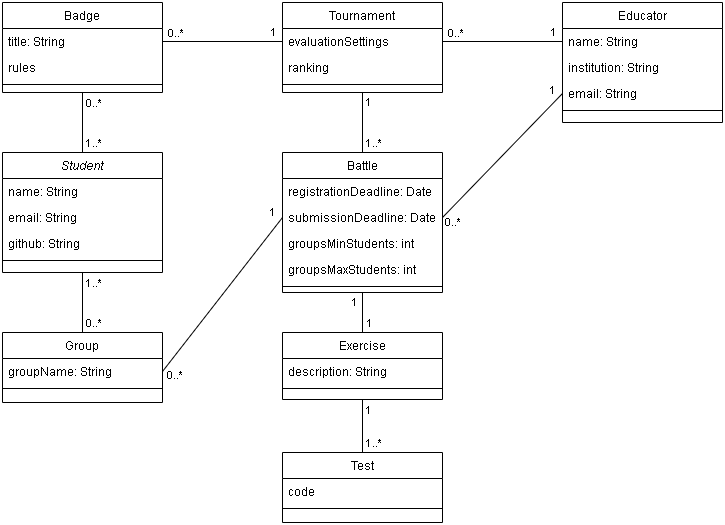
\includegraphics[width=0.8\textwidth]{Images/ClassDiagramRASD.png}
  \caption{Domain class diagram}
  \label{fig:ClassDiagram}
\end{figure}

\subsubsection{Statecharts}

\comment{Fare i diagrammi}

The CKB platform involves several key states and transitions to facilitate the seamless execution of code kata battles and tournaments. The primary states and transitions are described below:

\begin{enumerate}
    \item Tournament Lifecycle:
        \begin{itemize}
            \item States: Registration, Started, Closed
            \item Transitions: from Registration to Started (triggered when an educator starts a new tournament) and from Started to Closed (triggered when an educator decides to close the tournament)
        \end{itemize}

    \item Code Kata Battle Lifecycle:
        \begin{itemize}
            \item States: Created, Registration, Started, Consolidation, Closed
            \item Transitions: From Created to Registration Open (triggered when an educator creates a new code kata battle), From Registration Open to Started (occurs after the specified registration deadline), Started to Consolidation (when the battle ends, if required), Consolidation to Closed (when the evaluation ends)
        \end{itemize}

    \item Student Team Formation:
        \begin{itemize}
            \item States: Pending, Accepted, Rejected
            \item Transitions: From Pending to Accepted (occurs if the number of teammates that joined the group by accepting the invitation is within the range) of from Pending to Rejected (occurs when the number of teammates that accepted the invitation is lower than the minimum number, either at the end of the registration phase or after other students decline the invitation)
        \end{itemize}

    \item GitHub Integration:
        \begin{itemize}
            \item States: Repository Created, Workflow Established, Battle Closed
            \item Transitions: From Repository Created to Workflow Established (Students fork the GitHub repository and configure automated workflows) and Workflow Established to Battle Closed (Triggered when the battle's deadline expires)
        \end{itemize}

    \item Battle Score Update:
        \begin{itemize}
            \item States: Real-time Update, Consolidation Stage, Final Score
            \item Transitions: From Real-time Update to Consolidation Stage (Triggered after the submission deadline, indicating a transition to manual evaluation if necessary), from Consolidation Stage to Final Score (when the educator ends the manual evaluation).
        \end{itemize}

    
\end{enumerate}

\subsection{Product functions}

\comment{sostituire subsubsection con lista}

\subsubsection{Tournament Management}
 \begin{itemize}
    \item Create Tournament: educators can create new tournaments, specifying details such as description, start and end dates, and rules.
    \item Close Tournament: educators have the ability to close a tournament, signaling the end of the competition.
    \item Add Battles: educators can add battle to their tournaments or allows other educators to add them.
\end{itemize}

\subsubsection{Code Kata Battle Management}
 \begin{itemize}
    \item Create Code Kata Battle: educators can create code kata battles within a tournament, providing details such as the kata description, software project, build scripts, and scoring configurations.
    \item Set Battle Deadlines: educators can set registration and submission deadlines for each code kata battle.
\end{itemize}

\subsubsection{Student Interaction}
\begin{itemize}
    \item Registration and Team Formation: students can register for individual battles or form teams based on the specified team size limits. Teams are formed before the registration deadline.
\end{itemize}

\subsubsection{GitHub Integration}
\begin{itemize}
    \item Repository Creation: after the registration deadline, the platform automatically creates a GitHub repository for each team.
    \item Automated Workflow: students set up automated workflows using GitHub Actions to enable continuous integration. CI processes are triggered with each commit, updating the CKB platform in real-time.
\end{itemize}

\subsubsection{Scoring evaluation}
\begin{itemize}
    \item Automated Scoring: the platform automatically evaluates functional aspects, timeliness, and source code quality.
    \item Real-time Score Updates: scores are updated in real-time on the platform, visible to both students and educators.
    \item Manual Evaluation: educators can manually evaluate and assign personal scores, if required.
\end{itemize}

\subsubsection{Tournament Closure}
\begin{itemize}
    \item Close Tournament and Notify: educators can close a tournament, and the CKB platform notifies all students involved. Personal tournament scores are updated for each student.
\end{itemize}

\subsubsection{Gamification Badges}
\begin{itemize}
    \item Badge Creation: educators can create gamification badges associated with specific tournaments.
    \item  Badge Assignment: badges are automatically assigned based on predefined rules and student performance. Students and educators can view earned badges in a student's profile.
\end{itemize}

\subsubsection{Notification System}
\begin{itemize}
    \item Automatic Notifications: The platform automatically notifies students and educators about new tournaments, battles, and tournament closures. Notifications include important deadlines and updates.
\end{itemize}

\subsection{User characteristics}

\subsubsection{Educators}
\begin{itemize}
    \item Description: Educators play a crucial role in managing and overseeing the CKB platform. They are responsible for creating tournaments, defining code kata battles, and evaluating student submissions.
    \item Characteristics: Possess a deep understanding of software development concepts and practices. Have the authority to create, manage, and close tournaments. Able to assess student submissions based on various criteria, including code quality and adherence to coding practices.
\end{itemize}

\subsubsection{Students}
\begin{itemize}
    \item Description: Students are the primary users who participate in code kata battles and tournaments. They register for battles, form teams, and actively engage in coding exercises to demonstrate their software development skills.
    \item Characteristics: Have a basic understanding of programming languages and software development. Are motivated to improve their coding skills through practical challenges. Collaborate with team members during code kata battles to achieve common goals.
\end{itemize}


\subsection {Assumptions, dependencies and constraints}

\subsubsection{Assumptions}
\begin{itemize}
    \item The users (educators and students) have basic proficiency in using web-based platforms and are familiar with version control systems, such as Git.
    \item Educators have the necessary knowledge to create meaningful code kata battles, including defining test cases and scoring criteria
    \item Educators and students can connect to the Internet with their devices.
    \item Notification must arrive to connected users in one minute
    \item GitHub Account Requirement: students are required to have a GitHub account for participation, and the platform assumes that students have the necessary permissions to fork repositories.
    \item e-mail required
\end{itemize}

\subsubsection{Dependencies}
\begin{itemize}
    \item GitHub Integration: the CKB platform relies on GitHub for repository hosting and continuous integration processes.
    \item External APIs: Integration with external services may be required for additional functionalities, such as static code analysis tools.
    \item Internet Connectivity: Users (educators, students, administrators) need a reliable internet connection to interact with the CKB platform.
\end{itemize}

\subsubsection{Constraints}
\begin{itemize}
    \item Programming Languages: the platform supports a variety of programming languages for code kata battles, for example Java, Python, C, ...
    \item Browser Compatibility: the CKB platform is optimized for modern web browsers (e.g., Chrome, Firefox, Safari).
    \item Scalability: the platform must be designed to handle a scalable number of concurrent users during peak periods, such as registration deadlines.
     \item Security: the platform must adhere to security best practices to protect user data and prevent unauthorized access (sandboxing system since scripts can be malicious).
\end{itemize}

%------------------------------------------------------------------------------------------------------------------------------------------------
\clearpage
{\color{Black}{\section{Specific Requirements}}}
\label{sect:requirements}
\subsection{External interfaces}
\subsubsection{User interfaces}
\subsubsection{Hardware interfaces}
\subsubsection{Software interfaces}

\subsection{Functional Requirements}
\subsubsection{Use cases diagrams}
\subsubsection{Sequence diagrams}
\subsubsection{Requirements mapping}
\comment{Da fare alla fine}

\subsection{Performance requirements}
\begin{enumerate}
  \item \textbf{Response Time:} \\
  To ensure timely responsiveness for user interactions the platform should respond to user actions (e.g., loading pages, submitting forms) within a maximum of two seconds under normal load conditions.
  \item \textbf{Scalability:} \\
  To ensure the platform can handle an increasing number of users and data the platform should support concurrent access by at least 1000 users without significant degradation in performance, for up to 1000 battles simultaneously.
  \item \textbf{GitHub Integration:} \\
  GitHub repository creation, including code kata and automation setup, should take no longer than two minutes, also automated workflow triggers from GHA should result in platform updates within 1 minute of code submission, otherwise some students’ submission may be lost.
  \item \textbf{Automated Assessment and Consolidation Stage:} \\
  To ensure fast evaluation of code submissions, automated assessments (including code analysis and test execution) should complete within two minutes for a battle. Also, the platform should handle simultaneous automated assessments from multiple battles without queuing delays.
  \item \textbf{Notification System:} \\
  Notifications about battle and tournament updates need to be sent to every interested user in at most one minute.
  \item \textbf{Badges and Gamification:} \\
  To provide a continuous experience for badge assignment and visualization, they need to be assigned right after the end of each tournament and to the correct students. Also, their visualization on users’ profile should load instantaneously.
  \item \textbf{Security:} \\
  To ensure secure data handling and prevent unauthorized access user authentication and authorization processes should happen rapidly and the platform should do regular security inspections to identify and address potential vulnerabilities.
  \item \textbf{Data Storage and Retrieval:} \\
  To optimize data storage and retrieval processes, database queries for common operations should be fully optimized. Frequent backups are done to prevent data losses.
  \item \textbf{Reliability:} \\
  To ensure consistent and reliable performance, the platform should achieve 99.9\% uptime.
\end{enumerate}
These are criteria that CKB aims to achieve. Rigorous testing and continuous monitoring will be essential to meet and maintain these standards throughout the system’s lifecycle.

\subsection{Design constraints}
\subsubsection{Standard compliance}
\subsubsection{Hardware limitations}
\subsubsection{Any other constraint}

\subsection{Software system attributes}
\subsubsection{Reliability}
\subsubsection{Availability}
\subsubsection{Security}
\subsubsection{Maintainability}
\subsubsection{Portability}

%------------------------------------------------------------------------------------------------------------------------------------------------
\clearpage
{\color{Black}{\section{Formal Analysis Using Alloy}}}
\label{sect:alloy}
\subsection{Signatures}
In this chapter we report a formal analysis of the system performed with the specification language Alloy, along with the output of Alloy Analyzer, in order to check the correctness and coherence of the logical components of the system.\\
In this section, we list the signatures used in the formal analysis. Note that the description of the various components includes only the elements that are at interest in the formal analysis.

\begin{minted}{alloy}
open util/integer

sig Email,Name {}

sig Badge{
    tournament: one Tournament
}

sig Student{
    name: one Name,
    email: one Email,
    //The set of earned badges
    var badges: set Badge
}

sig Group{
    students: some Student
}

sig Educator{
    name: one Name,
    email: one Email
}

enum TournamentStatus{
    //The tournament has not been created yet
    NotCreatedYet,
    //The tournament has been created and it accepts subscriptions
    Subscription,
    //The tournament has started, students can solve battles within the tournament
    Started,
    //The tournament has been closed
    Closed
}

sig Tournament{
    creator: one Educator,
    var status: one TournamentStatus,
    //The set of students subscripted to the tournament
    var students: set Student
}

sig Battle{
    creator: one Educator,
    tournament: one Tournament,
    //Groups partecipating to the battle
    var groups: set Group
}
\end{minted}

\subsection{Time-independent facts}
Alloy facts allow the model to behave coherently with the real world. Facts can depend or not on the time evolution of the system: in this section, we report the static, time-independent facts.

\begin{minted}{alloy}
//All Emails correspond to at least a Student or an Educator
fact NoUnusedEmails{
    no e:Email | (no s:Student | s.email = e) and (no ed:Educator | ed.email = e)
}
//All Names correspond to at least a Student or an Educator
fact NoUnusedNames{
    no n:Name | (no s:Student | s.name = n) and (no ed:Educator | ed.name = n)
}

//All the students have unique Emails
fact UniqueEmailForStudents{
    no disj s1,s2:Student | s1.email = s2.email
}
//All the educators have unique Emails
fact UniqueEmailForEducators{
    no disj e1,e2:Educator | e1.email = e2.email
}
\end{minted}

\subsection{Time-dependent facts}
In this section we report all the facts that depend on the time evolution of the system. In particular, all the parameters listed with the keyword \textbf{var} can change over time, thus needing a time-dependent analysis.

\subsubsection{Tournaments}

\begin{minted}{alloy}
//Every Tournament is initially not created
fact BeginningNotCreatedYet{
    all t:Tournament | always(
    (t.status = NotCreatedYet implies historically t.status = NotCreatedYet) and
    (t.status != NotCreatedYet implies once t.status = NotCreatedYet) )
}

//Transition predicates
pred NotCreatedYetToSubscription[t:Tournament]{
    t.status = NotCreatedYet
    t.status' = Subscription
}
pred SubscriptionToStarted[t:Tournament]{
    t.status = Subscription
    t.status' = Started
}
pred StartedToClosed[t:Tournament]{
    t.status = Started
    t.status' = Closed
}

//All the changes in the tournament status follow the defined transitions
fact TransitionsFact{
    all t:Tournament | always( 
    (t.status = NotCreatedYet implies t.status'=t.status or 
    NotCreatedYetToSubscription[t]) and
    (t.status = Subscription implies t.status'=t.status or SubscriptionToStarted[t]) and
    (t.status = Started implies t.status'=t.status or StartedToClosed[t]) and
    (t.status = Closed implies t.status'=t.status))
}

//All the tournaments eventally close
fact TournamentsClose{
    all t: Tournament | eventually t.status = Closed
}

//The students can subscribe only in the Subscription phase
fact SubscriptionsInTournament{
    all t:Tournament | always(
    (t.status = NotCreatedYet implies #t.students = 0 ) and
    (t.students' != t.students implies t.status' = Subscription))
}
\end{minted}

\subsubsection{Groups and Battles}

\begin{minted}{alloy}
//All the groups partecipate to a battle
fact NoUnusedGroups{
    all g:Group | eventually one b:Battle | g in b.groups
}

//Groups are created only for individual battles
fact NoRepeatedGroups{
    always( no disj b1,b2:Battle | #(b1.groups & b2.groups)>0 )
}

//Groups can partecipate only if the tournament has started
fact GroupsBattleChangesHappenAfterStart{
    all b:Battle | always(
    (b.tournament.status = NotCreatedYet implies #b.groups = 0)
    and
    (b.groups' != b.groups implies b.tournament.status' = Started))
}

//Students can partecipate only in one group for each battle
fact NoStudentsTowGroupsSameBattle{
    all b:Battle | always(
    no disj g1,g2:Group | g1 in b.groups and g2 in b.groups
    and #(g1.students & g2.students)>0)
}

//Groups can partecipate only if all their components are subscripted to the tournament
fact SubscriptionToPartecipate{
    all b:Battle | always(all g:Group | g in b.groups implies
    (all s:Student | s in g.students implies s in b.tournament.students))
}

//Educators cannot partecipate as Students to their battles
fact NoEducatorsRegisteredAndCreate{
    always(no b:Battle | b.creator.email in b.groups.students.email)
}
\end{minted}

\subsubsection{Badges}

\begin{minted}{alloy}
//The set of badges of each student can change
pred ChangedBadgesSet[s:Student,b:Badge]{
    b not in s.badges
    s.badges' = s.badges + b
}

//The set of badges increments only
fact NoSubtractedBadges{
    all s:Student | always( all b:Badge |
    (b in s.badges implies b in s.badges'))
}

//Badges can be earned only when a tournament they are subscribed to closes
fact BadgesWhenTournamentCloses{
    all s:Student | once #s.badges = 0 and always(
    all b:Badge | ChangedBadgesSet[s,b] implies 
    (s in b.tournament.students and StartedToClosed[b.tournament]))
}
\end{minted}

%------------------------------------------------------------------------------------------------------------------------------------------------
\clearpage
{\color{Black}{\section{Effort Spent}}}
\label{sect:effort}
Provide here information about how much effort each group member spent in working at this document. We would appreciate details here.

%\begin{center}
%    \begin{tabular}{|c|c|}
%\hline
%    \textbf{Author} & \textbf{Hours spent} \\
%\hline
%    Annechini Alessandro & 1 \\
%\hline
%Filippi Nicole & 1 \\
%\hline
%Fiorentini Riccardo & 1 \\
%\hline
%\end{tabular}
%\end{center}

\begin{table}[h!]
  \centering
  \begin{tabular}{|c|c|}
    \hline
    Chapter & Hours spent \\
    \hline
    1 & 2\\
    \hline
    2 & 4\\
    \hline
    3 & 2\\
    \hline
    4 & 14\\
    \hline
  \end{tabular}
  \caption{Alessandro Annechini}
  \label{tab:Alessandro_Annechini_hours}
\end{table}

\begin{table}[h!]
  \centering
  \begin{tabular}{|c|c|}
    \hline
    Chapter & Hours spent \\
    \hline
    1 & 8\\
    \hline
    2 & 4\\
    \hline
    3 & 8\\
    \hline
    4 & 2\\
    \hline
  \end{tabular}
  \caption{Nicole Filippi}
  \label{tab:Nicole_Filippi_hours}
\end{table}

\begin{table}[h!]
  \centering
  \begin{tabular}{|c|c|}
    \hline
    Chapter & Hours spent \\
    \hline
    1 & 2\\
    \hline
    2 & 14\\
    \hline
    3 & 2\\
    \hline
    4 & 2\\
    \hline
  \end{tabular}
  \caption{Riccardo Fiorentini}
  \label{tab:Riccardo_Fiorentini_hours}
\end{table}


%------------------------------------------------------------------------------------------------------------------------------------------------
%\clearpage
%\addcontentsline{toc}{section}{References}
%\bibliographystyle{plain}
%\bibliography{main}
\clearpage
{\color{Black}{\section{References}}}
\label{sect:references}

\begin{enumerate}
    \item Inspirational sites similar to our web application:
    \begin{itemize}
           \item \url{https://codecombat.com}
           \item \url{https://www.codingame.com}
           \item \url{https://codebattle.hexlet.io}
           \item \url{https://www.codebattle.in}
   \end{itemize}
    \item DrawIO, tool used for sequence diagrams and development diagrams. \textsc{url}: \url{https://www.drawio.com}
    \item Moqups, tool used for web application's mockups. \textsc{url}: \url{https://moqups.com}
    \item Specification document: \texttt{"Assignment RDD AY 2023-2024"}
    \item DD sample from A.Y. 2022-2023
    \item \LaTeX, used to redact the document. Documentation:\\
   \url{https://www.latex-project.org/help/documentation/}
   \item Overleaf, \LaTeX \textbf{ }online editor. \textsc{url}:
   \url{https://www.overleaf.com/}
   
    
\end{enumerate}
%------------------------------------------------------------------------------------------------------------------------------------------------

\end{document}
